\subsection{Iterator}
Viene utilizzato per permette ad una classe client di effettuare l'accesso sequenziale agli elementi di un aggregato, senza esporre l'implementazione dell'oggetto.

\begin{figure}[ht]
    \centering
    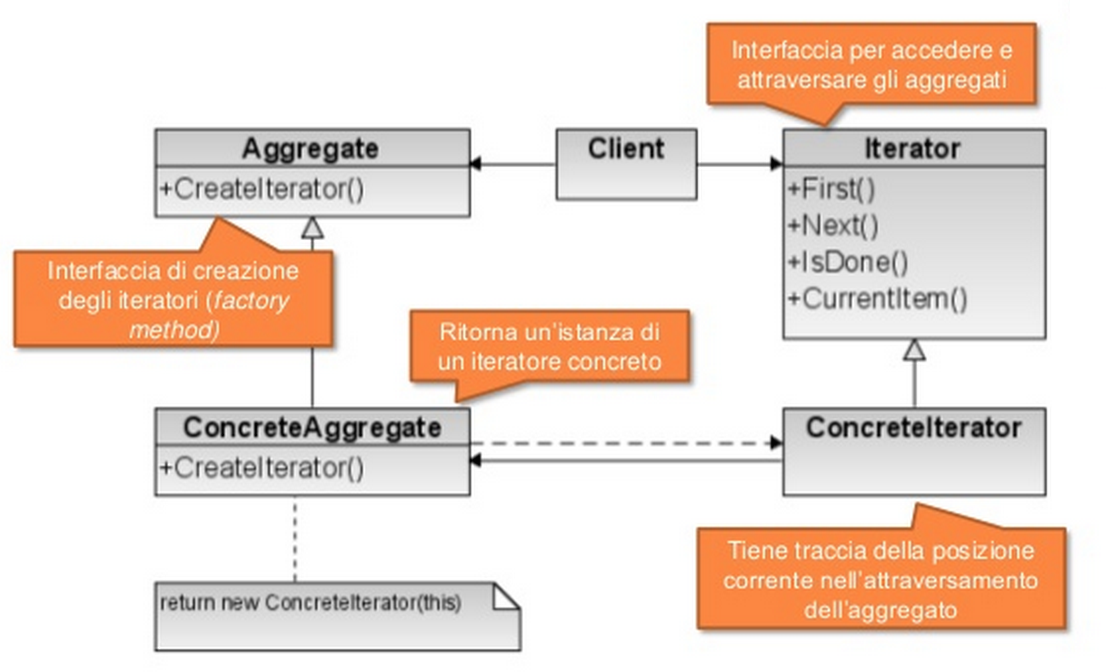
\includegraphics[width=0.8\textwidth]{immagini/iterator.png}
    \caption{Iterator}
\end{figure}
\FloatBarrier

Nonostante il concetto di iteratore sia di per se semplice, quando viene implementato è necessario fare alcune considerazioni riguardo la logica di attraversamento e al comportamento quando vengono aggiunti o tolti dei componenti durante l'uso dell'iteratore.
Difatti, il controllo dell'iterazione può essere fatto sia dal client, invocando un metodo dell'iteratore, sia dall'iteratore stesso in modo automatico. Allo stesso modo, l'algoritmo di attraversamento può essere definito dall'aggregato oppure dall'iteratore stesso.

\subsubsection{Casi tipici}
\begin{itemize}
\item \`{E} necessario accedere agli elementi di una collezione senza sapere come sono memorizzati;
\item C'è bisogno di poter attraversare la collezione più molte, anche in modo concorrente;
\item Si vuole fornire un'inferfaccia uniforme di attraversamento;
\item Ci possono essere più modi per attraversare la stessa collezione.
\end{itemize}